\documentclass[12pt,a4paper]{article}

% Encoding and language
\usepackage[utf8]{inputenc}
\usepackage{lmodern}
\usepackage{svg}
\usepackage[backend=biber, style=ieee]{biblatex}
\addbibresource{yourfile.bib} 
% Layout and spacing
\usepackage[a4paper,margin=2.5cm,top=20mm]{geometry}
\usepackage{fullpage}
\usepackage{setspace}
\setlength\parindent{0pt}

% Section depth
\setcounter{secnumdepth}{5}
\setcounter{tocdepth}{5}

% Code and listings
\usepackage{listings}
\usepackage{xcolor}
\lstset{
  basicstyle=\ttfamily\small,
  backgroundcolor=\color{gray!10},
  frame=single,
  breaklines=true,
  postbreak=\mbox{\textcolor{red}{$\hookrightarrow$}\space},
  keywordstyle=\color{blue},
  commentstyle=\color{gray},
  stringstyle=\color{orange}
}

% Math and tables
\usepackage{amsmath}
\usepackage{booktabs}
\usepackage{siunitx}
\usepackage{pdfpages}
% Graphics and figures
\usepackage{graphicx}
\usepackage{float}
\usepackage{subcaption}
\usepackage{tikz}
\usepackage{svg}
\usepackage{pdflscape}
\usepackage{pdfpages}

% Referencing and hypertext
\usepackage{hyperref}
\hypersetup{
  pdftitle = {DNOD_Documentation},
  pdfsubject = {Workshop Project Documentation},
  pdfauthor = {Odin Hasson, Benjamin Schalk},
  colorlinks = false
}
\usepackage{prettyref}
\usepackage{url}

% Bibliography - commented out until .bib file is available
% \usepackage[backend=biber,style=numeric]{biblatex}
% \addbibresource{quellen.bib}  % Make sure this points to the correct .bib file

% Header and footer
\usepackage{fancyhdr}
\usepackage{lastpage}
\pagestyle{fancy}
\fancyhf{}
\renewcommand{\headrulewidth}{0.5pt}
\renewcommand{\footrulewidth}{0.5pt}
\lhead{Odin Hasson, Benjamin Schalk}
\chead{PBE}
\rhead{17.06.2025}
\fancyfoot[C]{Page \thepage{} of \pageref{LastPage}}
\setlength{\headsep}{0.8cm}
\setlength{\footskip}{0.7cm}

% Custom TODO notes
\usepackage{xargs}
\usepackage[colorinlistoftodos,prependcaption,textsize=tiny]{todonotes}
\newcommandx{\unsure}[2][1=]{\todo[linecolor=red,backgroundcolor=red!25,bordercolor=red,#1]{#2}}
\newcommandx{\change}[2][1=]{\todo[linecolor=blue,backgroundcolor=blue!25,bordercolor=blue,#1]{#2}}
\newcommandx{\info}[2][1=]{\todo[linecolor=black,backgroundcolor=black!25,bordercolor=black,#1]{#2}}
\newcommandx{\improvement}[2][1=]{\todo[linecolor=purple,backgroundcolor=purple!25,bordercolor=purple,#1]{#2}}
\newcommandx{\thiswillnotshow}[2][1=]{\todo[disable,#1]{#2}}

% Misc
\usepackage{circuitikz}
\usepackage{glossaries}
\usepackage{blindtext}
\usepackage{algpseudocodex}
\usepackage{algorithm}
\usepackage{enumitem}
\usepackage{pgffor}       % add this in preamble if not already there
\renewcommand*{\pageautorefname}{page} 
% Extra heading depth
\usepackage{hyperref}

\makeatletter
\newcommand\subsubsubsection{\@startsection{paragraph}{4}{\z@}%
  {-3.25ex \@plus -1ex \@minus -.2ex}%
  {1.5ex \@plus .2ex}%
  {\normalfont\normalsize\bfseries}}
\newcommand\subsubsubsubsection{\@startsection{subparagraph}{5}{\z@}%
  {-3.25ex \@plus -1ex \@minus -.2ex}%
  {1.5ex \@plus .2ex}%
  {\normalfont\normalsize\bfseries}}
\makeatother

\begin{document}

\begin{center}
\begin{minipage}{0.1\textwidth}
% Empty minipage
\end{minipage}%
\hfill
\begin{minipage}{0.9\textwidth}
\centering
% Empty minipage
\end{minipage}
\end{center}

\begin{center}
\textbf{\large Project Documentation} \\[0.5em]
\textbf{Digital Night Observation Device} \\[0.5em]
\vspace{1em}
\end{center}

\begin{center}
\begin{tabular}{rl}
\textbf{Autor:} & Odin Hasson, Benjamin Schalk \\
\textbf{Datum:} & 17.6.2025 \\
\end{tabular}
\end{center}         




\begin{figure}[H]
    \centering
    \includegraphics[width=1\linewidth]{images/logo.png}

    \label{fig:enter-label}
\end{figure}



\newpage


    
    
\section{Introduction}

\subsection{Group members}

\subsubsection*{Odin Hasson}
\begin{minipage}[c]{0.3\textwidth}
    \centering
    \includegraphics[width=\linewidth]{images/odin.png}

    \label{fig:odin-hasson}
\end{minipage}%
\hfill
\begin{minipage}[c]{0.58\textwidth}
    As the team leader, I oversaw the allocation of team members, ensuring that each individual was assigned tasks best suited to their expertise and the project's needs. My primary technical contributions centered on the hardware development of our project, with a particular focus on designing the foundational circuitry. Additionally, I collaborated closely with Benjamin Schalk in the co-design of the PCB, ensuring both functionality and efficiency. Beyond these core responsibilities, I provided support across various aspects of the design process and took sole responsibility for all manufacturing and implementation related to 3D printing and 3D printed components.
\end{minipage}
\subsubsection*{Benjamin Schalk}
\begin{minipage}[c]{0.3\textwidth}
    \centering
    \includegraphics[width=\linewidth]{images/benni.png}
    \captionof{figure}{Benjamin Schalk}
    \label{fig:benjamin-schalk}
\end{minipage}%
\hfill
\begin{minipage}[c]{0.58\textwidth}
    In this project, my primary responsibility was to develop the software. In addition to the software development, I actively contributed to the hardware development, collaborating closely with Odin Hasson. I contributed heavily to the design of the PCB.
\end{minipage}

\newpage
\subsection{Project Overview}
The Digital Night Observation Device (henceforth referred to as ``DNOD'' in this document) consists, at its most fundamental level, of a microcontroller, a digital display, and a NoIR camera. The microcontroller utilizes an AI chip (also known as a KPU) to process video and perform facial recognition. The camera is a simple digital unit that outputs video directly to the microcontroller board. The board processes the video signal and forwards the modified signal to the display.


%EasyEda PRO, MaixPy IDE, kflash_gui, Shar3r, Fusion, Visual Studio Code, Overleaf, lucidchart
\newpage
\section{Design}
\subsection{High Level Architecture (Hardware)}
\autoref{fig:hardware-high-level} visualizes the high-level hardware architecture. Light blue boxes represent hardware components within the Sipeed M1W module, while light yellow boxes indicate input and output elements. Note that the diagram does not show the entire system: subcircuits are required to support each I/O element and the M1W module itself are omitted for clarity. Additionally, the battery used to power DNOD is not shown.
\begin{figure}[H]
    \centering
    \includesvg[width=0.75\linewidth]{images/hardware-high-level}
    \caption{High level architecture (Hardware)}
    \label{fig:hardware-high-level}
\end{figure}
\newpage
\subsection{High Level Architecture (Software)}
\autoref{fig:software-high-level} depicts the high-level software architecture. The reference config stores important const values such as image ratio, color depth, and other important information. In the depiction, blue boxes reference functions, and excluding the initial reference to the config, the rest of the functions loop. Using the config the user can easily adjust settings such as bitrate, which version of the MLM\footnote{\textbf{M}achine \textbf{L}earning \textbf{M}odel} should be used, aswell as graphical settings such as upscaling or edge sharpening in order to increase visual quality, or sacrifice visual quality for perfomance.


\begin{figure}[H]
    \centering
    \includesvg[width=0.65\linewidth]{images/software-high-level}
    \caption{High level architecture (Software)}
    \label{fig:software-high-level}
\end{figure}
\newpage
\subsection{Project Housing}
\subsubsection{PCB, Camera, and Display Housing}
We decided to place the PCB, camera, and display within the same housing to save space. The housing effectively “stacks” each core component vertically. Each individual component is separated from the others to ensure proper isolation. The display and the camera are connected via 24 Pin flat ribbon cable connectors. Additionally, the case includes a dovetail, so that the device can be mounted to a helmet. The software Shapr3D and Fusion was used to design the housing

\begin{figure}[H]
  \centering
  \begin{minipage}[b]{0.48\linewidth}
    \centering
    \includegraphics[width=\linewidth]{images/pcb_housing_front.png}
    \caption{PCB, display, and camera housing when viewed from the front}
    \label{fig:pcb_housing_front}
  \end{minipage}
  \hfill
  \begin{minipage}[b]{0.48\linewidth}
    \centering
    \includegraphics[width=\linewidth]{images/pcb_housing_rear.png}
    \caption{PCB, display, and camera housing when viewed from the rear}
    \label{fig:pcb_housing_rear}
  \end{minipage}
\end{figure}


\subsubsection{Battery Housing}
The battery housing is quite simple, it contains a slot for a DC jack port and, at the bottom, small dovetails onto which the battery connectors can slide.
\begin{figure}[H]
    \centering
    \includegraphics[width=0.5\linewidth]{images/battery_housing.png}
    \caption{Battery housing}
    \label{fig:battery_housing}
\end{figure}

\subsection{Circuit Design}
Our base circuit is derived from elements of the SIPEED Maixduino, a microcontroller built around the SIPEED M1 module. The SIPEED Maixduino is well-documented, and its complete circuit schematic is readily available online. Utilizing both the official documentation and our own technical knowledge, we designed an alternative version that retains and enhances the specific features of the Maixduino relevant to our application.

% SVG figures - commented out because files don't exist
% Replace with placeholder text or actual figures when available

\subsection{Circuit Components}

\subsubsection{K210 Circuit}
The K210 circuit forms the core of the processing system, incorporating the AI-capable microcontroller and its supporting components. See page \pageref{pdfpage1} for the schematic overview.

\subsubsection{LCD Connector Circuit}
The LCD connector circuit interfaces with the display module, handling both data transmission and power delivery. See page \pageref{pdfpage2} for the schematic overview.

\subsubsection{Camera Connector Circuit}
The camera connector circuit provides the interface between the NoIR camera module and the main processing unit. This circuit ensures proper signal integrity and power delivery to the camera module. See page \pageref{pdfpage3} for the schematic overview.

\subsubsection{USB-C Port Circuit}
The USB-C port circuit handles both power input and data communication with external devices. See page \pageref{pdfpage4} for the schematic overview.

\subsubsection{GPIO Circuit}
The General Purpose Input/Output (GPIO) circuit provides expandable connection points for additional sensors or peripherals. See page \pageref{pdfpage5} for the schematic overview.

\subsubsection{SD Card Circuit}
The SD card circuit provides expandable storage capabilities for the device, allowing for data logging and firmware storage. See page \pageref{pdfpage6} for the schematic overview.


\subsubsection{DC Power Circuit}
The DC power circuit handles the main power distribution throughout the device, ensuring all components receive appropriate voltage levels. See page\pageref{pdfpage7} for the schematic overview.

\subsubsection{Camera Power Circuit}
The camera power circuit manages the power supply requirements for the camera module, providing stable voltage regulation and filtering to ensure optimal image quality. See page \pageref{pdfpage8} for the schematic overview.

\subsubsection{ISP Download}
This circuit allows in-system programming of a microcontroller via UART using an ESP32. See \pageref{pdfpage9} for the schematic overview.

\subsubsection{DAC Circuit}
The Digital-to-Analog Converter (DAC) circuit enables the conversion of digital signals from the microcontroller to analog outputs when required. See page\pageref{pdfpage10} for the schematic overview.

\subsubsection{ESP-32}
The ESP-32 was originally included as we intended to include Bluetooth/WiFi capabilities to our projects, but couldn't achieve that goal due to time constraints. See page \pageref{pdfpage11} for the schematic overview

\subsubsection{Miscellaneous Circuits}
Additional supporting circuits provide various auxiliary functions such as status indicators, reset functionality, and system monitoring. See page \autoref{pdfpage12} for the schematic overview.

{
  \pagestyle{empty}  % disable fancyhdr headers/footers

  \foreach \n in {1,...,12} {
    \clearpage
    \phantomsection
    \label{pdfpage\n}
    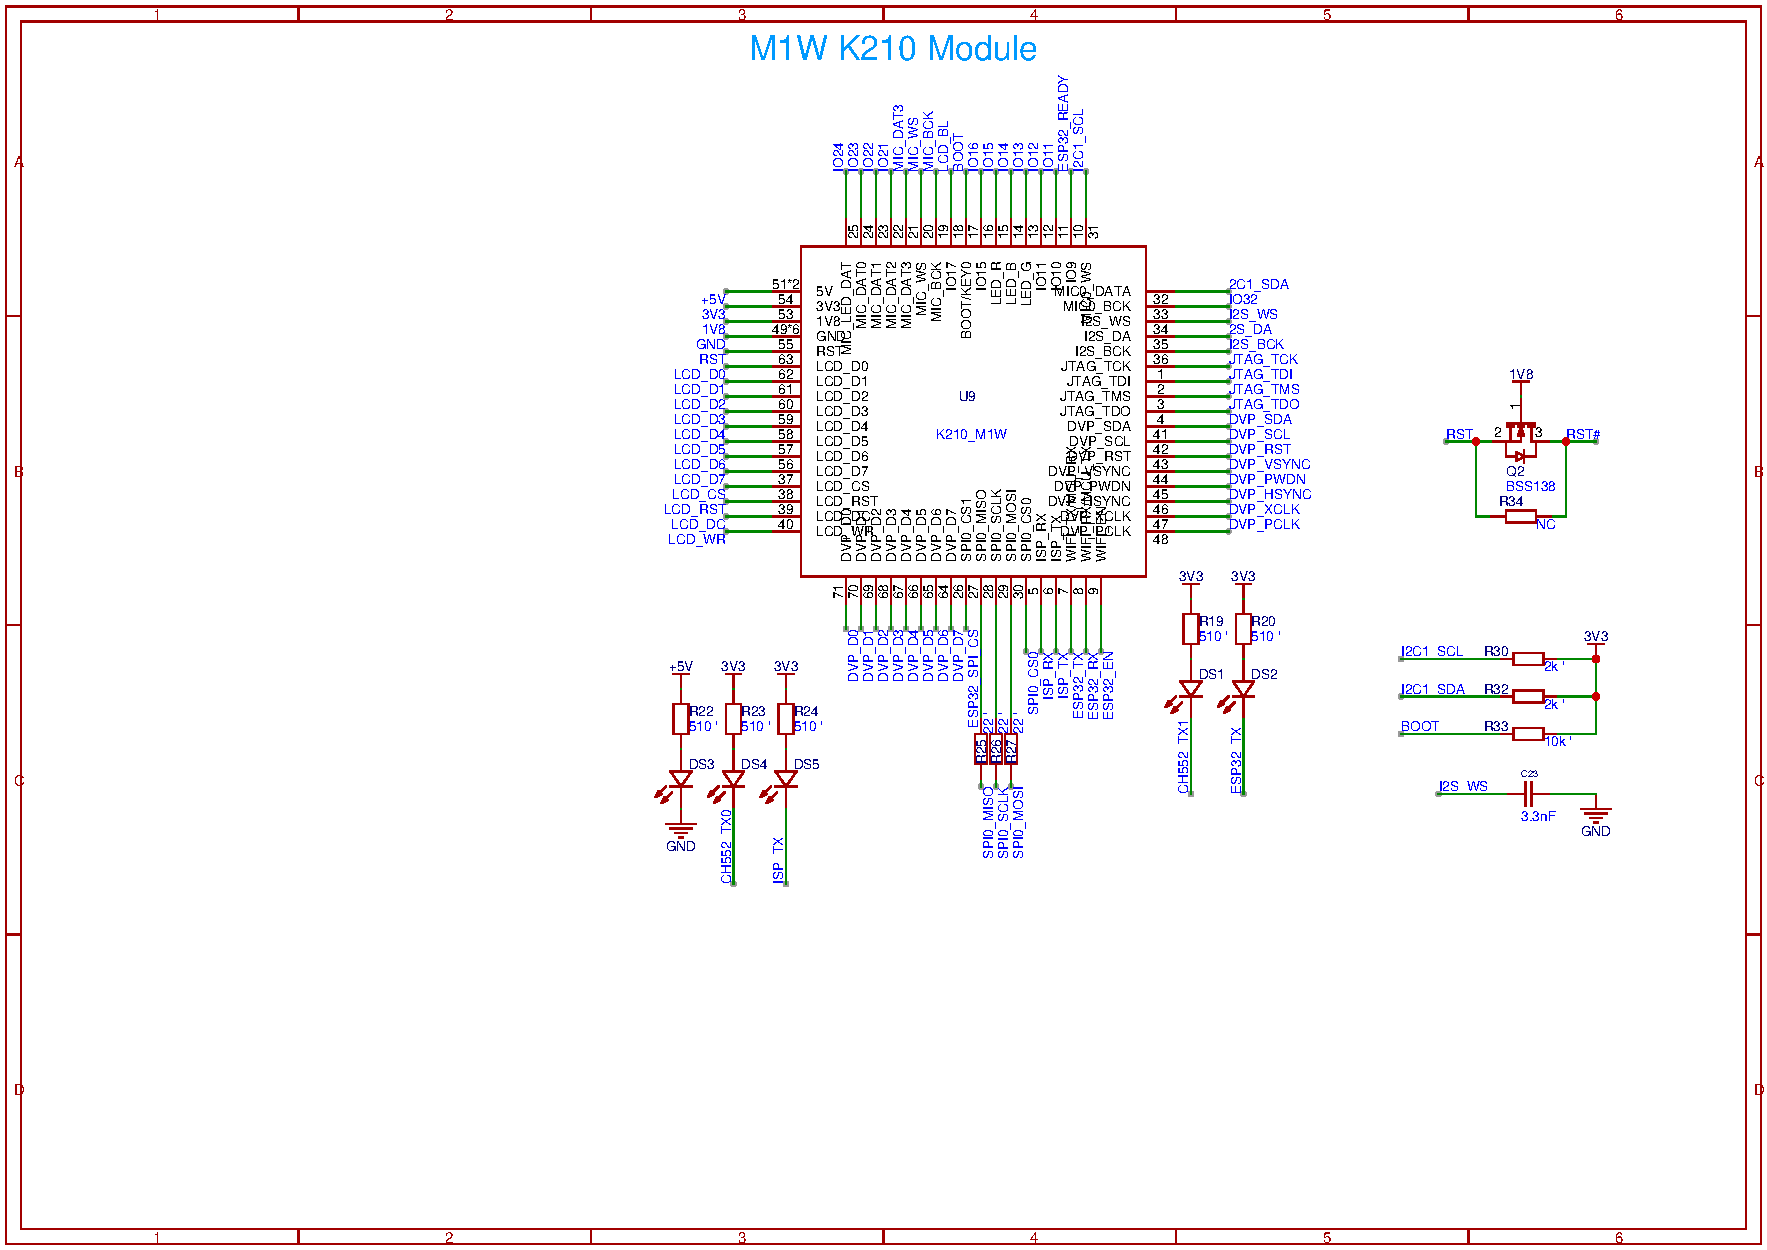
\includepdf[
      pages=\n,
      scale=0.90,
      pagecommand={},
      fitpaper=true
    ]{subcircuit.pdf}
  }

  \clearpage
  \pagestyle{fancy}  % restore your original header/footer
}
\newpage
\subsection{PCB Design}
To design our PCB, we used the software EasyEda Pro. We did two interations, We made two iterations, the second iteration is depicted here.
\subsubsection{Top Layer}

The layout of the top layer can be found in \autoref{pcbpage1}. It illustrates the primary routing and placement of components on the upper surface of the PCB.

\subsubsection{Bottom Layer}

The layout of the bottom layer is shown in \autoref{pcbpage2}, highlighting the ground planes and any signal routing on the reverse side.


\newpage
{
  \pagestyle{empty}  % Disable headers/footers on these pages

  \phantomsection
  \label{pcbpage1}
  \includepdf[
    pages=1,
    landscape=true,
    scale=0.8,
    pagecommand={},
    fitpaper=false
  ]{pcb.pdf}

  \phantomsection
  \label{pcbpage2}
  \includepdf[
    pages=2,
    landscape=true,
    scale=0.8,
    pagecommand={},
    fitpaper=false
  ]{pcb.pdf}
}

\newpage
\section{Production}
\subsection{Programming}
The Sipeed M1 K210 module can be flashed using the software known as KFlash, and then, using Sipeed’s proprietary

\subsubsection{SmartFaceDisplay 1.0}
Our SmartFaceDisplay 1.0 is a compact solution for real-time face recognition with a camera, AI module, and display. As soon as the device is powered on, the camera starts and continuously sends images to the onboard "KPU" accelerator. The YOLO algorithm analyzes each frame for faces and automatically overlays detected areas with colored bounding boxes. The final image, including these markings, is displayed live on the screen, while the current frame rate (FPS) is shown in the corner.

\subsubsubsection*{Core Features}
\begin{itemize}[left=0pt]
  \item \textbf{Automatic Face Detection:} The AI scans each camera image for faces and draws rectangular frames around them.
  \item \textbf{Live Feedback:} Detection results and performance data (frames per second) are shown directly on the LCD.
  \item \textbf{Easy Startup:} Using the MaixPy IDE, the Python script can be quickly run on the K210 board; the model is loaded directly from flash memory at startup.
\end{itemize}

\subsubsubsection*{Optional Features}
\begin{itemize}[left=0pt]
  \item \textbf{Image Filters (Convolution):} A sharpening or edge detection filter can optionally be activated (e.g., \texttt{img.conv3(edge)} or \texttt{img.conv3(sharp)}).
  \item \textbf{Upscaling Mode:} For more detailed displays, the image can be enlarged before rendering (\texttt{img.resize(384, 288)}), but this requires more RAM.
  \item \textbf{Configurable Thresholds:} Confidence parameters of the YOLO model can be adjusted during initialization to modify detection accuracy and sensitivity.
  \item \textbf{Alternative Models:} Instead of the preinstalled face model, other YOLO models (e.g., for detecting license plates, objects, or people in specific contexts) can also be loaded and ran.
\end{itemize}

All of these extras can be flexibly enabled or disabled by commenting or uncommenting a few lines in the script. This makes the SmartFaceDisplay 1.0 not only ready to use out of the box but also ideal for experimentation and adaptation to specific use cases — whether for visitor counting, access control, or as a demonstrator for AI-based image processing.

\subsection{PCB Production}
\subsubsection{JLCPCB Manufacturing}
The printed circuit board was manufactured in Hong Kong by JLCPCB\cite{jlcpcb2025}, components were sourced from mouser.at\cite{mouser2025} and LCSC\cite{lcsc2025}
\subsubsection{Use of soldering oven}
To solder the chips and smaller ICs, we used the soldering oven found in our workshop. To solder using the soldering oven, soldering paste must be applied to all contact points, before the chip is placed.

\begin{figure}[htbp]
  \centering
  \begin{minipage}[b]{0.48\linewidth}
    \includegraphics[width=\linewidth]{images/oven1.jpeg}
    \caption{PCB being prepared for the soldering oven}
    \label{fig:enter-label}
  \end{minipage}%
  \hfill
  \begin{minipage}[b]{0.48\linewidth}
    \includegraphics[width=\linewidth]{images/oven2.jpeg}
    \caption{PCB in oven being soldered}
    \label{fig:pcb_in_over}
  \end{minipage}
\end{figure}
\newpage

\subsubsection{Hand soldering}
To solder the resistors and capacitors, we soldered by hand.
\begin{figure}[H]
    \centering
    \includegraphics[width=0.5\linewidth]{images/hand_soldering.jpeg}
    \caption{An example of some of the hand-done soldering.}
    \label{fig:enter-label}
\end{figure}


\newpage
\section{Feedback}
\subsection{What went well}
The design of all digital aspects such as circuits, software, and the PCB went well.
\subsection{What went bad}
\begin{enumerate}
    \item Soldering the PCB was very difficult due to the small component size.
    \item Certain things that we had ordered took forever to arrive and caused delays.
\end{enumerate}

\section{Final Product}
\autoref{fig:helmet} shows our application of the digital night observation device. We mounted to battery to the back of the helmet, and the main board to the mounting point at the front of the helmet
\begin{figure}
    \centering
    \includegraphics[width=1\linewidth]{images/final.png}
    \caption{Digital night observation device mounted to a helmet}
    \label{fig:helmet}
\end{figure}
\newpage
\appendix
\section{Addendum: Daniel Liew}
Originally, our group consisted of three members. Daniel Liew disappeared after the initial week of the summer semester and never returned. Since then, he has been officially expelled. As he only attended workshop once after the begin of the summer semester and was never seen again, we removed him from the development cycle. This was not done immediately; however, after being informed of his expulsion and receiving no response to our attempts to contact him, we decided to remove him from the project.


\newpage
% Bibliography section commented out until .bib file is available
% \printbibliography
\section*{Used Software and Services}
The following software tools and services were used during this project:
\begin{enumerate}
  \item \textbf{EasyEDA Pro}. Available at: \url{https://easyeda.com/}. Accessed: 2025-06-17.
  \item \textbf{Shapr3D}. Available at: \url{https://www.shapr3d.com/}. Accessed: 2025-06-17.
  \item \textbf{Fusion 360}. Available at: \url{https://www.autodesk.com/products/fusion-360/}. Accessed: 2025-06-17.
  \item \textbf{JLCPCB}. Available at: \url{https://jlcpcb.com/}. Accessed: 2025-06-17.
  \item \textbf{LCSC Electronic Components Online}. Available at: \url{https://www.lcsc.com/}. Accessed: 2025-06-17.
  \item \textbf{Mouser Electronics Austria}. Available at: \url{https://www.mouser.at/}. Accessed: 2025-06-17.
\end{enumerate}
\end{document}